\documentclass[onecolumn, draftclsnofoot,10pt, compsoc]{article}
\usepackage{graphicx}
\usepackage{url}
\usepackage{setspace}
\usepackage{parskip}
\usepackage{geometry}
\geometry{textheight=9.5in, textwidth=7in}

% 1. Fill in these details
\def \CapstoneTeamName{AgBizClimate}
\def \CapstoneTeamNumber{26}
\def \GroupMemberOne{	Thomas Noelcke}
\def \GroupMemberTwo{	Shane Barrantes}
\def \GroupMemberThree{	Shengpei Yuan}
\def \CapstoneProjectName{ Linking Seasonal Weather Data to AgBizClimate\texttrademark}
\def \CapstoneSponsorCompany{ Oregon State University}
\def \CapstoneSponsorPerson{ Clark Seavert}

% 2. Uncomment the appropriate line below so that the document type works
\def \DocType{		Software Requirements Document
				%Requirements Document
				%Technology Review
				%Design Document
				%Progress Report
				}

\newcommand{\NameSigPair}[1]{\par
\makebox[2.75in][r]{#1} \hfil 	\makebox[3.25in]{\makebox[2.25in]{\hrulefill} \hfill		\makebox[.75in]{\hrulefill}}
\par\vspace{-12pt} \textit{\tiny\noindent
\makebox[2.75in]{} \hfil		\makebox[3.25in]{\makebox[2.25in][r]{Signature} \hfill	\makebox[.75in][r]{Date}}}}
% 3. If the document is not to be signed, uncomment the RENEWcommand below
%\renewcommand{\NameSigPair}[1]{#1}

%%%%%%%%%%%%%%%%%%%%%%%%%%%%%%%%%%%%%%%
\begin{document}
\begin{titlepage}
    \pagenumbering{gobble}
    \begin{singlespace}
        \hfill
        % 4. If you have a logo, use this includegraphics command to put it on the coversheet.
        %\includegraphics[height=4cm]{CompanyLogo}
        \par\vspace{.2in}
        \centering
        \scshape{
            \huge CS Capstone \DocType \par
            {\large\today}\par
            \vspace{.5in}
            \textbf{\Huge\CapstoneProjectName}\par
            \vfill
            {\large Prepared for}\par
            \Huge \CapstoneSponsorCompany\par
            \vspace{5pt}
            {\Large\NameSigPair{\CapstoneSponsorPerson}\par}
            {\large Prepared by }\par
            Group\CapstoneTeamNumber\par
            % 5. comment out the line below this one if you do not wish to name your team
            %\CapstoneTeamName\par
            \vspace{5pt}
            {\Large
                \NameSigPair{\GroupMemberOne}\par
                \NameSigPair{\GroupMemberTwo}\par
                \NameSigPair{\GroupMemberThree}\par
            }
            \vspace{20pt}
        }
        \begin{abstract}

        \end{abstract}
    \end{singlespace}
\end{titlepage}
\newpage
\pagenumbering{arabic}
\tableofcontents
% 7. uncomment this (if applicable). Consider adding a page break.
\listoffigures 
\newpage
%\listoftables
\clearpage

% 8. now you write!
\section{Introduction}
		\subsection{Purpose}
		This SRS describes the requirements and specifications of the AgBizClimate\texttrademark web application. This document will explain the functional features of this web application. This includes the interface details, design constraints and considerations such as performance characteristics. This SRS is intended out outline how we will proceed with the development of the \textit{AgBizClimate} system.\\

		\subsection{Scope}
			This project is a part of a much larger AgBiz Logic\texttrademark program. However, the purpose of this project is to add a short term climate tool to the \textit{AgBizClimate} module. This limits the scope of the project to the \textit{AgBizClimate} Module. Additionally, we will only be adding the short term climate data tool as the long term climate data tool already exists.\\

		\subsection{Definitions, Acronyms and Abbreviations}
			REST - Representaional State Transfer, This is a type of architecture that manages the state of the program. This is esspecially populare in web development.\\
			API- Application Programming Interface. This is a peice of softwared that allows a connection to another peice of software providing some sort of service.\\
			NWCTB - Northwest Climate Toolbox. This is the database we will be connecting to that will provide the short term climate data we plan to use.\\
			Climate Scenario - This is a theoretical calculation of yields, inputs and of the overall budget for one situation based on the climate data.\\
			SQL Database - This is a relational database that makes storing and accessing data easy.\\

			\renewcommand\refname{\vskip -1cm}
		\subsection{References}

		\nocite{*}
    \bibliographystyle{IEEEtran}
    \bibliography{IEEEabrv,References}


		\subsection{Overview}
			Seasonal climate is one of the essential factors that affects agricultural production. As a module of \textit{AgBiz Logic}, \textit{AgBizClimate} delivers essential information about climate change to farmers, and help professionals to develop management pathways that best fit their operations under a changing climate. This project aims to link the crucial seasonal climate data from the Northwest Climate Toolbox database to \textit{AgBiz Logic} so that it can provide changes in net returns of crop and livestock enterprises through powerful graphics and tables. \\
			Currently \textit{AgBizClimate} has a long-term climate tool but no such tool exists for short term climate data. We will implement a tool to extract short-term climate data from the Northwest Climate Toolbox database, display it to the user and allow the user to adjust crop and livestock yields or quality of products sold and, production inputs. Moreover, a landing tool will be developed to allow users to switch between short-term seasonal tool and long-term climate data tool.\\
\section{Overall Description}
	\subsection {Product Functions}
				\textit{AgBizClimate} is a web based decision tool that will allow users to gain specific insight on how localized climate data for the next seven months will affect their crop and livestock yields or quality of products sold and production inputs. The \textit{AgBizClimate} tool will allow users to input their location (state, county) and a budget for the specific crop or livestock enterprise. \textit{AgBizClimate} will select climate data for the next seven months for that location and provide graphical data showing temperature and precipitation. Users will then be able to change yields or quality of product sold by a percentage they think these factors will affect and modify production inputs. Finally the tool will calculate the net returns.\\

	\subsection{User Characteristics}
		\textit{AgBizClimate} users can be split into two subgroups, agricultural producers and climate researchers. The first subgroup, agricultural users who use this product tend to be between fifty and sixty years old of mixed gender. Their educational background ranges from high school to the completion of college. The primary language this group uses is English, but there are some Spanish users as well. Most of the users in this group tend to have novice computational skills. The primary domain for these users is agricultural and business management. Most agricultural producers who use this product are motivated by the potential profit that the decision tool \textit{AgBizClimate} could potentially offer. The second subgroup, climate researchers range from ages twenty to forty and are of mixed gender. The educational background for most climate researchers  exceed the postgraduate level with their primary language being English. These users generally have advanced computational skills and are motivated by the easily accessible climate and weather data.\\

	\subsection{Constraints}
		There are several key constraints that this product has to work within. The first constraint is that we only have access to two data parameters from the North West Climate Tool box, precipitation and temperature. Secondly, we only have access to their data via the NWCTB API which could have additional restrictions such as limited usage per day, mislabeled data, or poor documentation. Thirdly, we don’t have access to any of the hardware that \textit{AgBizClimate} is exists on as it is being managed by a third party. This will prevent us from improving the hardware or cause roadblocks if their servers are having issues. Lastly, we are limited to using the languages Python and JavaScript since we are integrating our product into an already existing project.\\

	\subsection {Assumptions and Dependencies}
		We are assuming that the Northwest Climate Toolbox is a functional API that will allow us to pull location based temperature and precipitation data. This data will most likely come in the form of a text body of which we will then format into a JSON object and store in a Mongo database for future use. Due to the fact that we are writing an addition to an existing project we do not need to interact with the user budgets as these have already been defined. This fact extends to the calculations portion of the \textit{AgBizClimate} product. Our team will simply be accessing data via the NWCT API, then format the data, store the data, and hand the data over to the tool while will provide some additional front end support.\\

\section{Specific Requirements}
This section contains all of the functional and quality requirements of the \textit{AgBizClimate} System. We will give detailed description of what's being added to the \textit{AgBiz Logic} system along with the features we will implement.\\
    \subsection{External Interface Requirements}
		This section provides a detailed description of all inputs into and outputs from the short term climate tool for the \textit{AgBizClimate} system. This section will also provide descriptions for the hardware, software and communication interfaces. Additionally we will provide detailed prototypes for the user interface for the short term climate data tool.\\
        \subsubsection{User Interface}
					When the user first navigates to \textit{AgBizClimate} from the \textit{AgBiz Logic} main page the user will be directed to a landing page. This landing page will allow the user to either select the existing long term climate tool or the short term climate tool that we will be developing. On this page there will be a brief description of the tool and what does. This description will also describe the difference between the long term climate data tool and the short term data climate tool. Below this description will be two buttons one to run the long term climate data tool and one to run the short term climate data tool. Clicking the long term climate data tool button will take you to the long term climate data tool page. Clicking the short term climate data tool button will take you to the short term climate data tool page. A prototype of this page is shown below in figure 3.1.\\
					
					\begin{figure}
						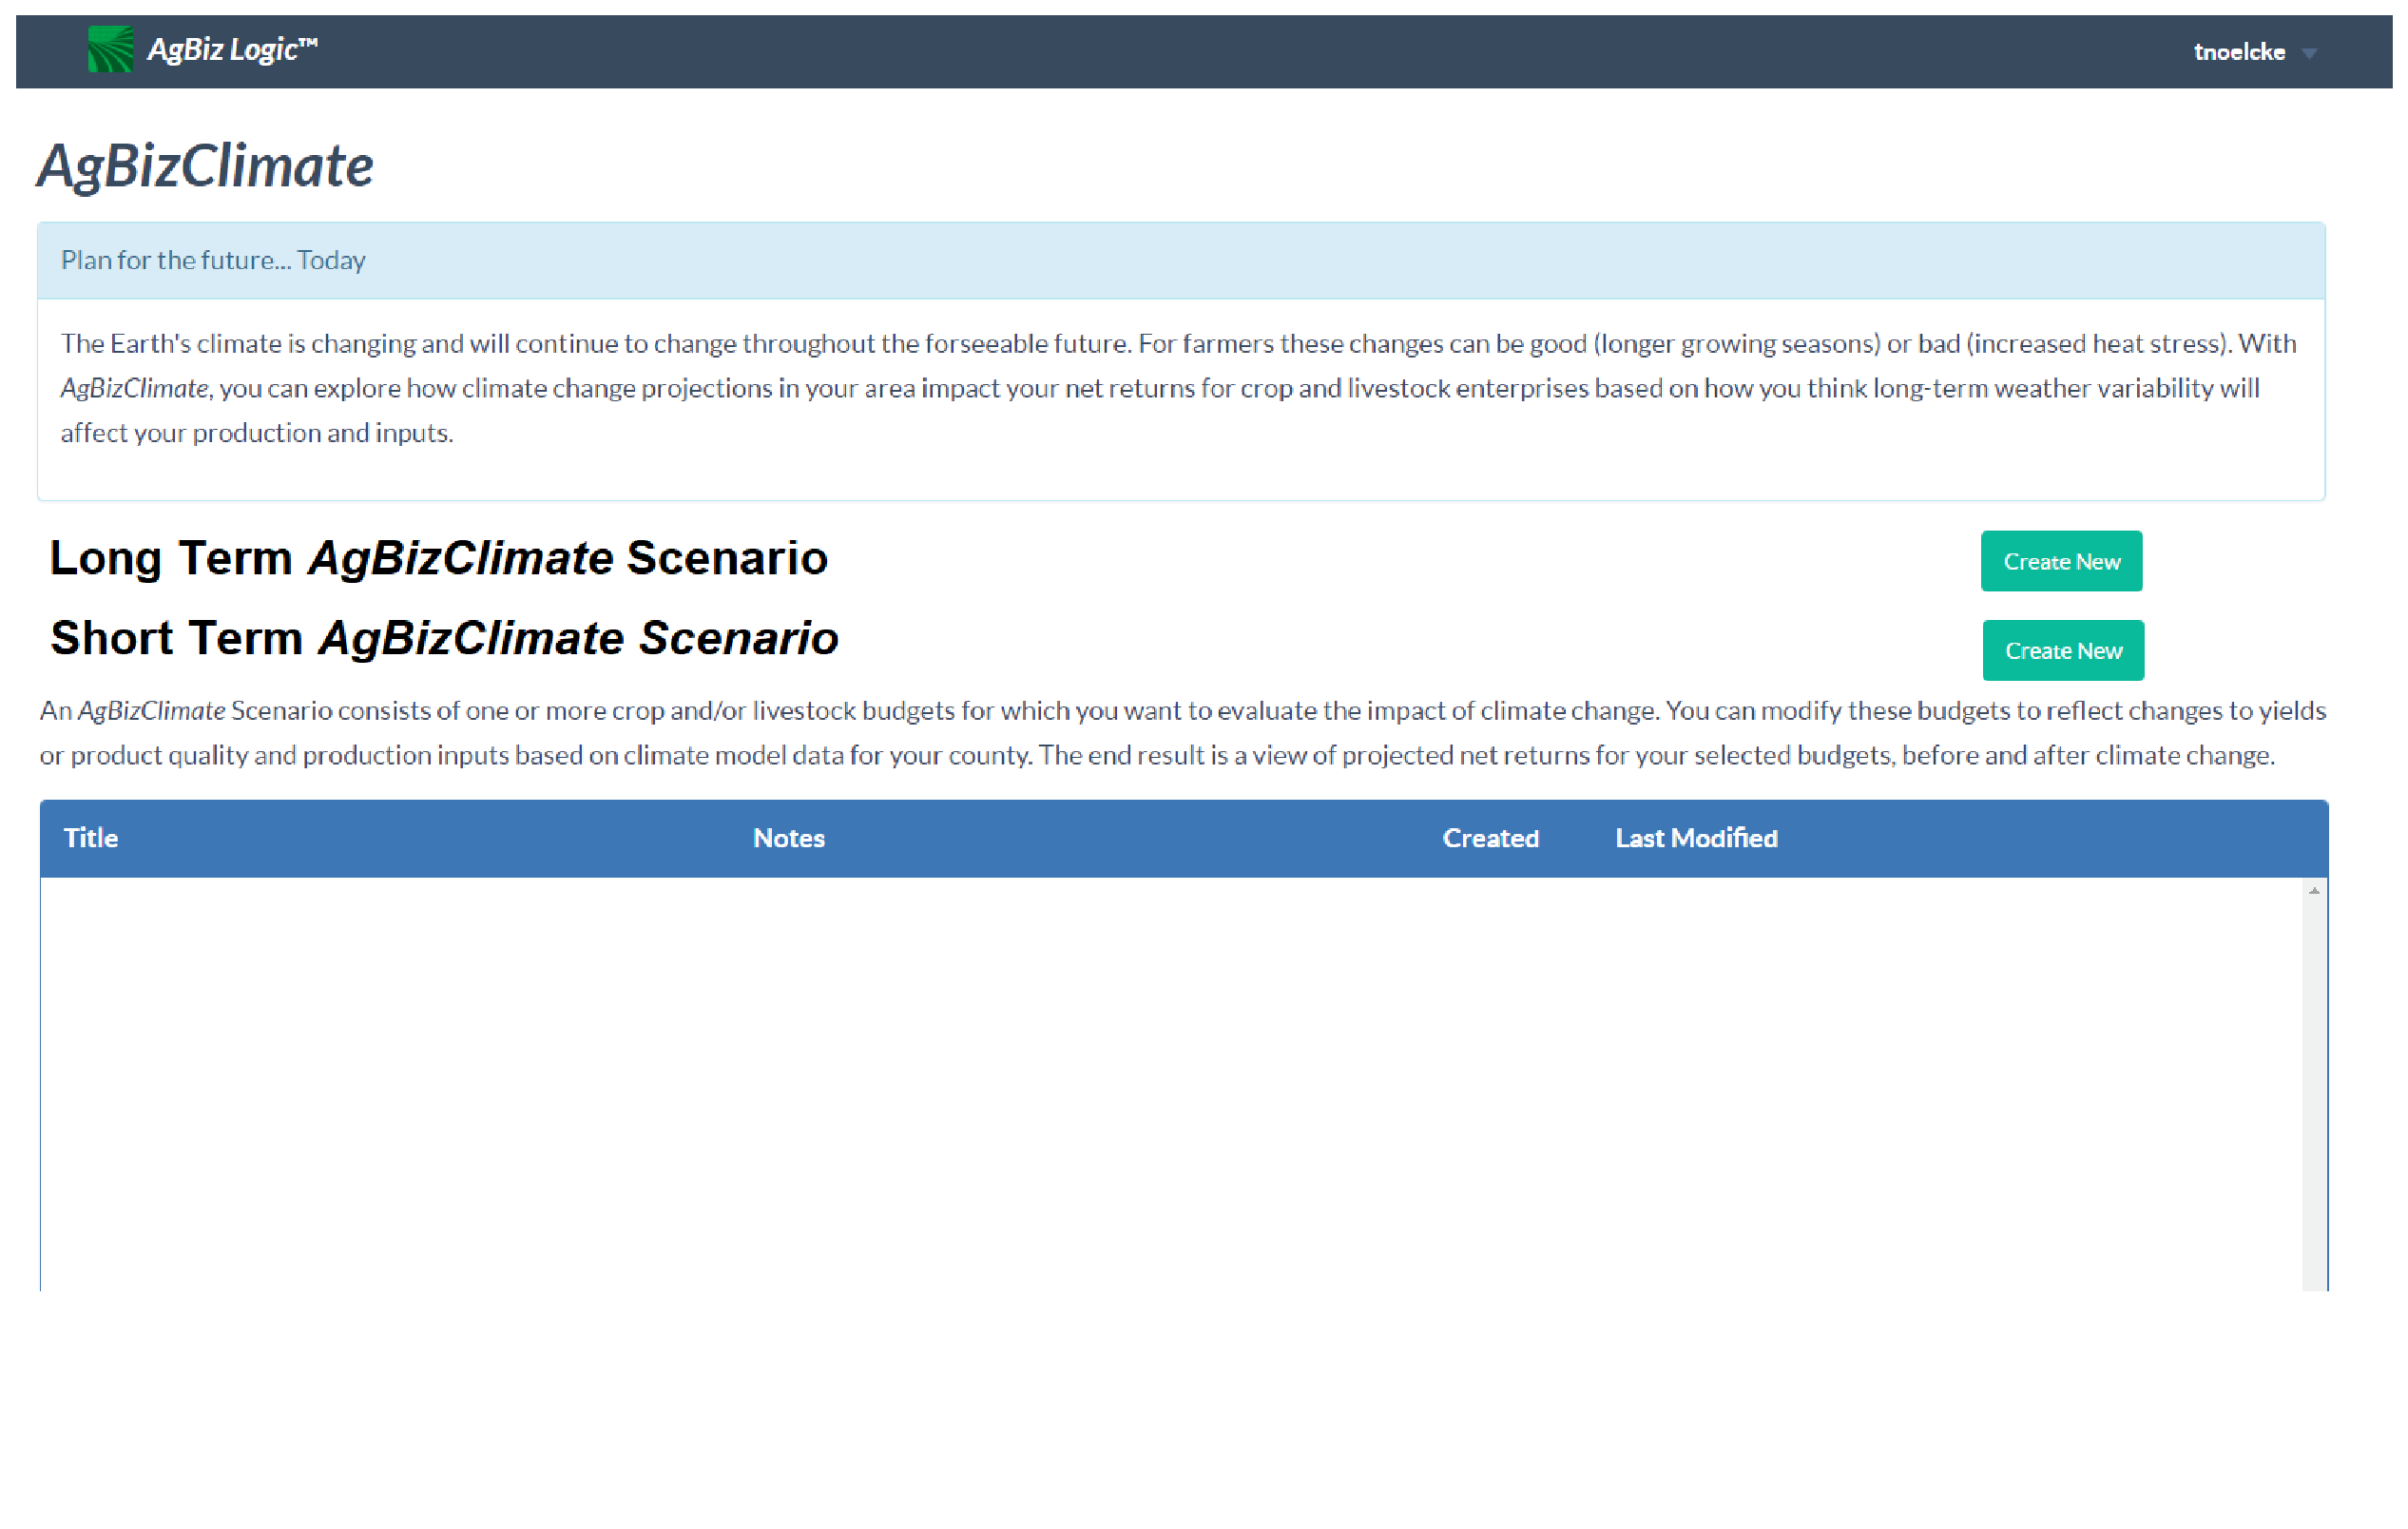
\includegraphics[width=\linewidth]{Figures/LandingPage.eps}
						\caption{Landing Page}
						\label{figure3.1}
					\end{figure}
					

					After clicking on the short term climate data tool page you will be directed to a page that will allow you to create a new climate scenario. This page will allow the user to chose which budgets they would like to adjust and make notes about this scenario. This page also allows them to cancel or delete the scenario they are currently working on. A prototype for this page is shown below in figure 3.2.\\
					
					\begin{figure}
						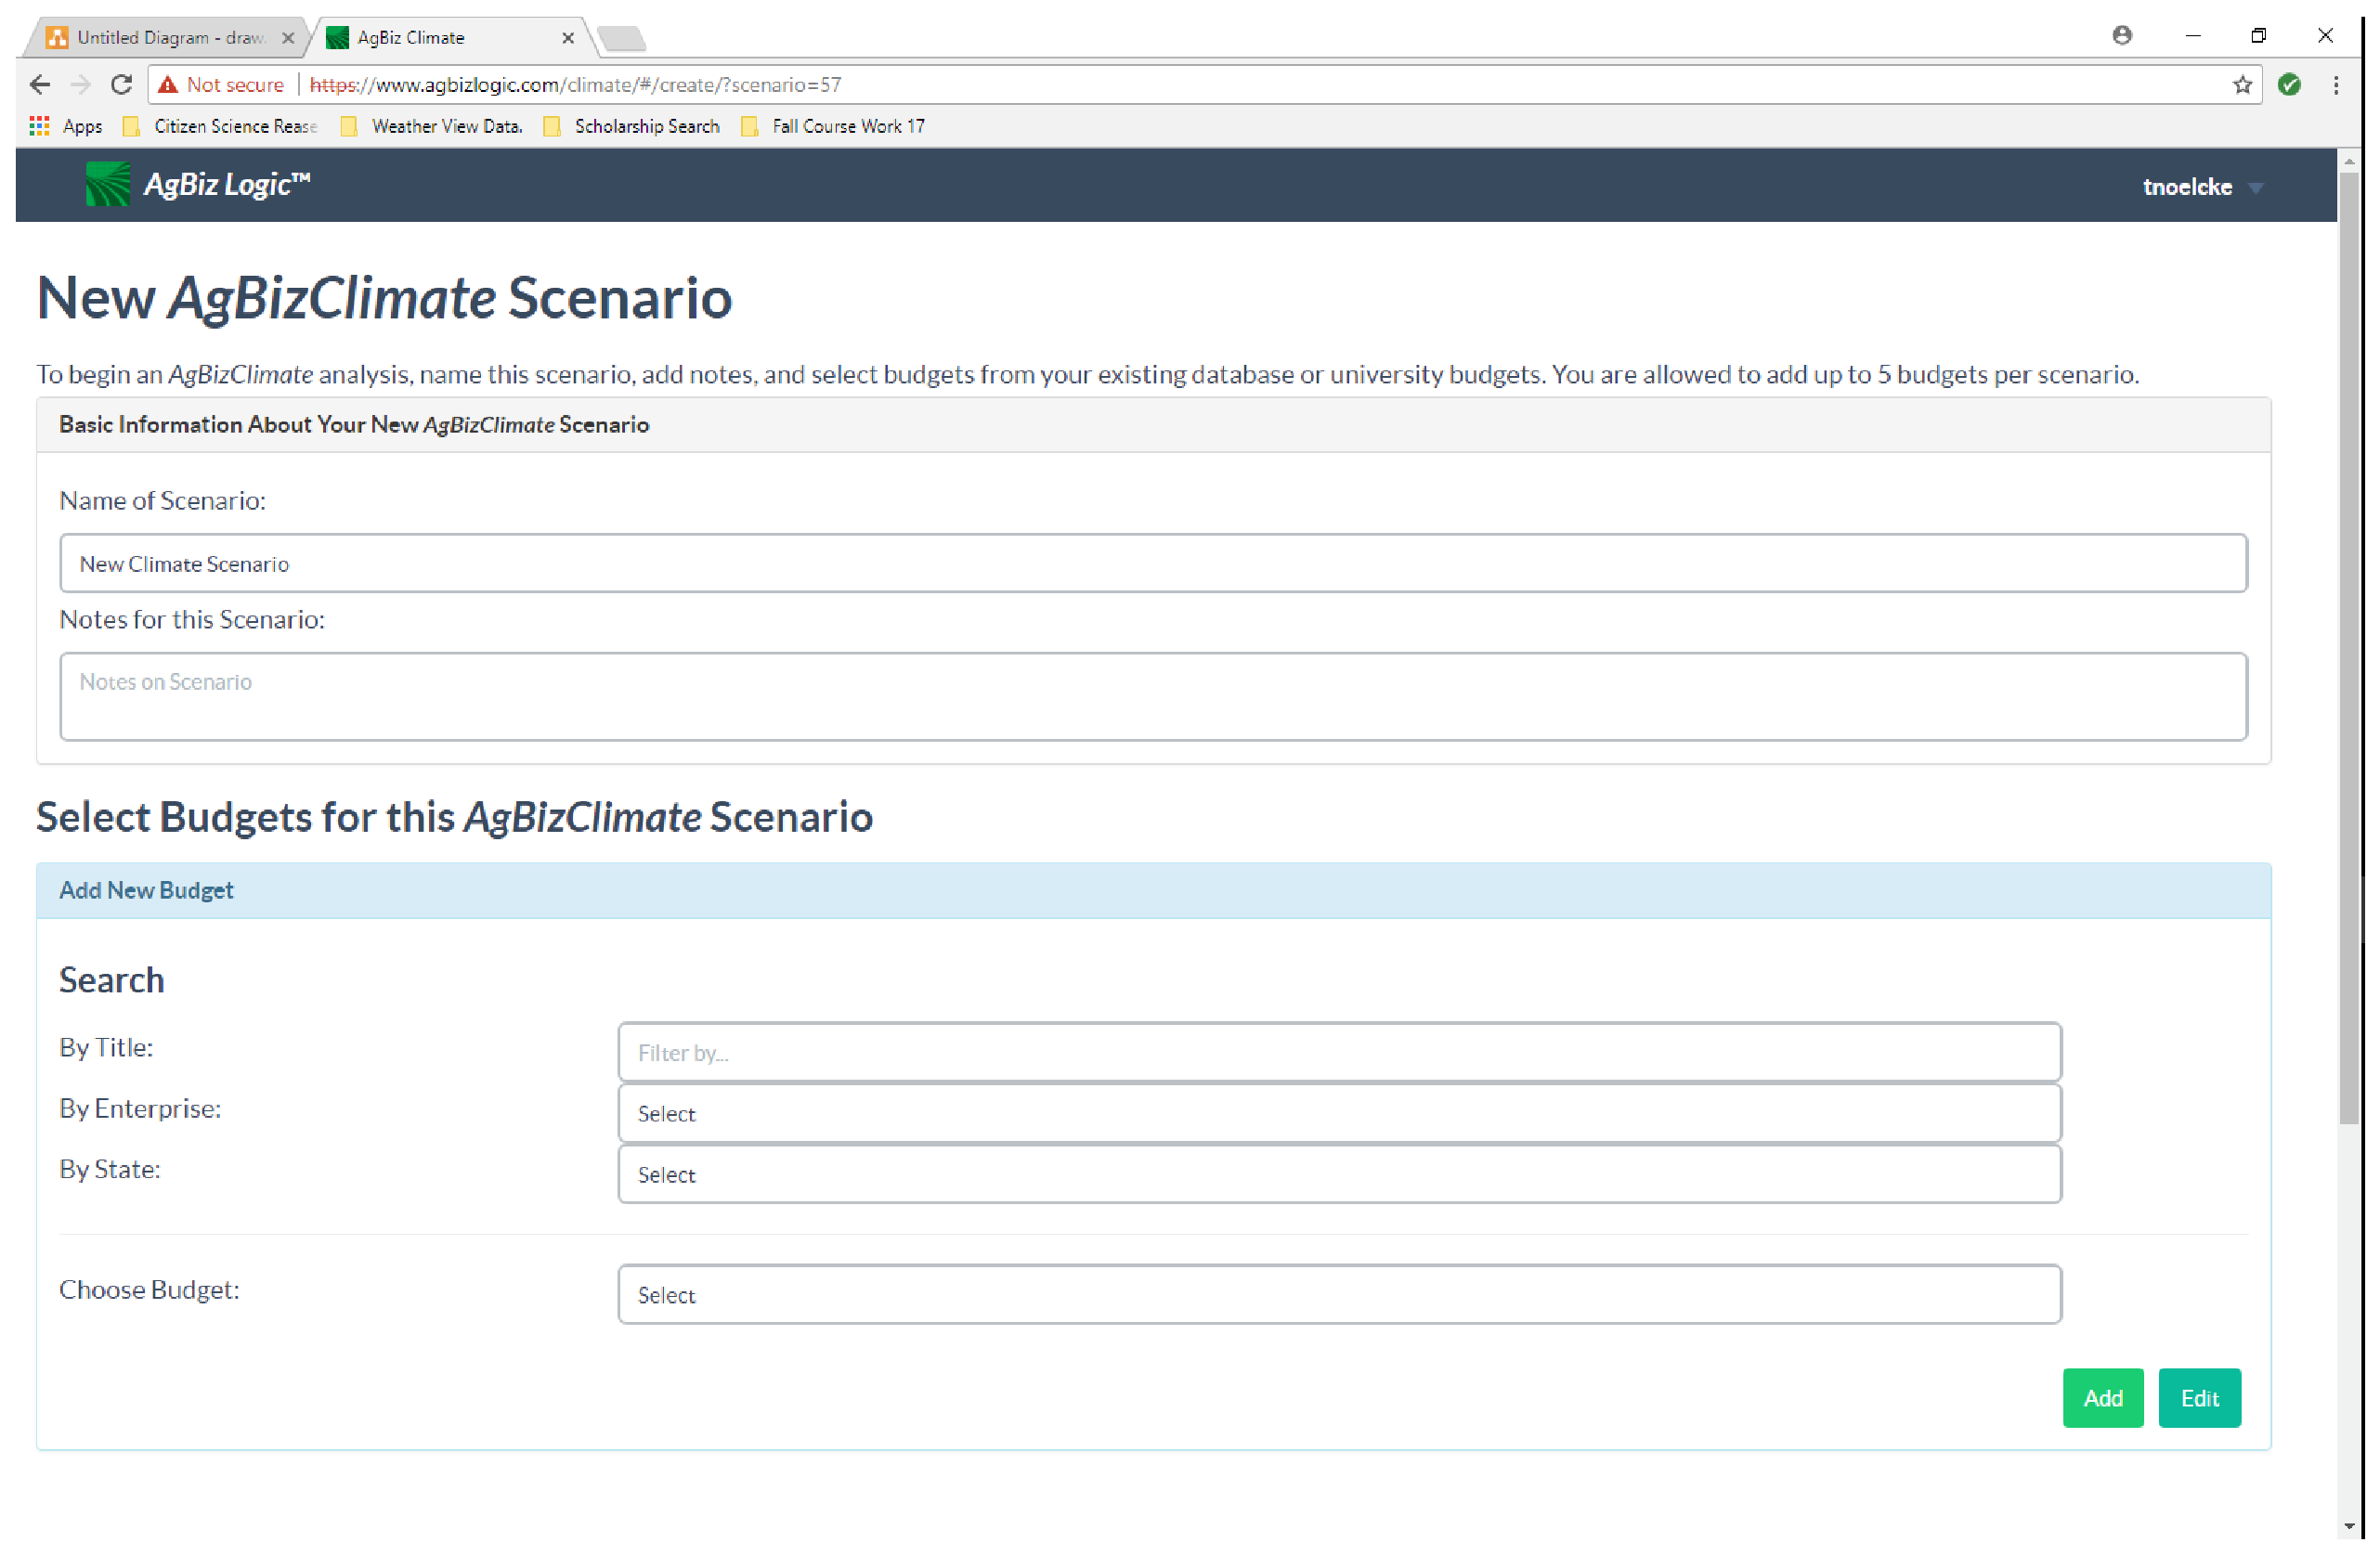
\includegraphics[width=\linewidth]{Figures/ClimateScenario.eps}
						\caption{Allows user to select budgets and make notes}
						\label{figure3.2}	
					\end{figure}

					Once the user Selects their budgets, makes notes on the scenario and clicks continue the will be redirected to a page where they will be prompted to enter their location. This page will take a county and a sate as input. This page will have a drop down menu for the state and the county. Before the user can enter a County they will be forced to enter a state. Once a state is entered the county drop down menu will auto populate and the user will be allowed to enter a county. A prototype of this page is shown below in figure 3.3.\\
					
					\begin{figure}
						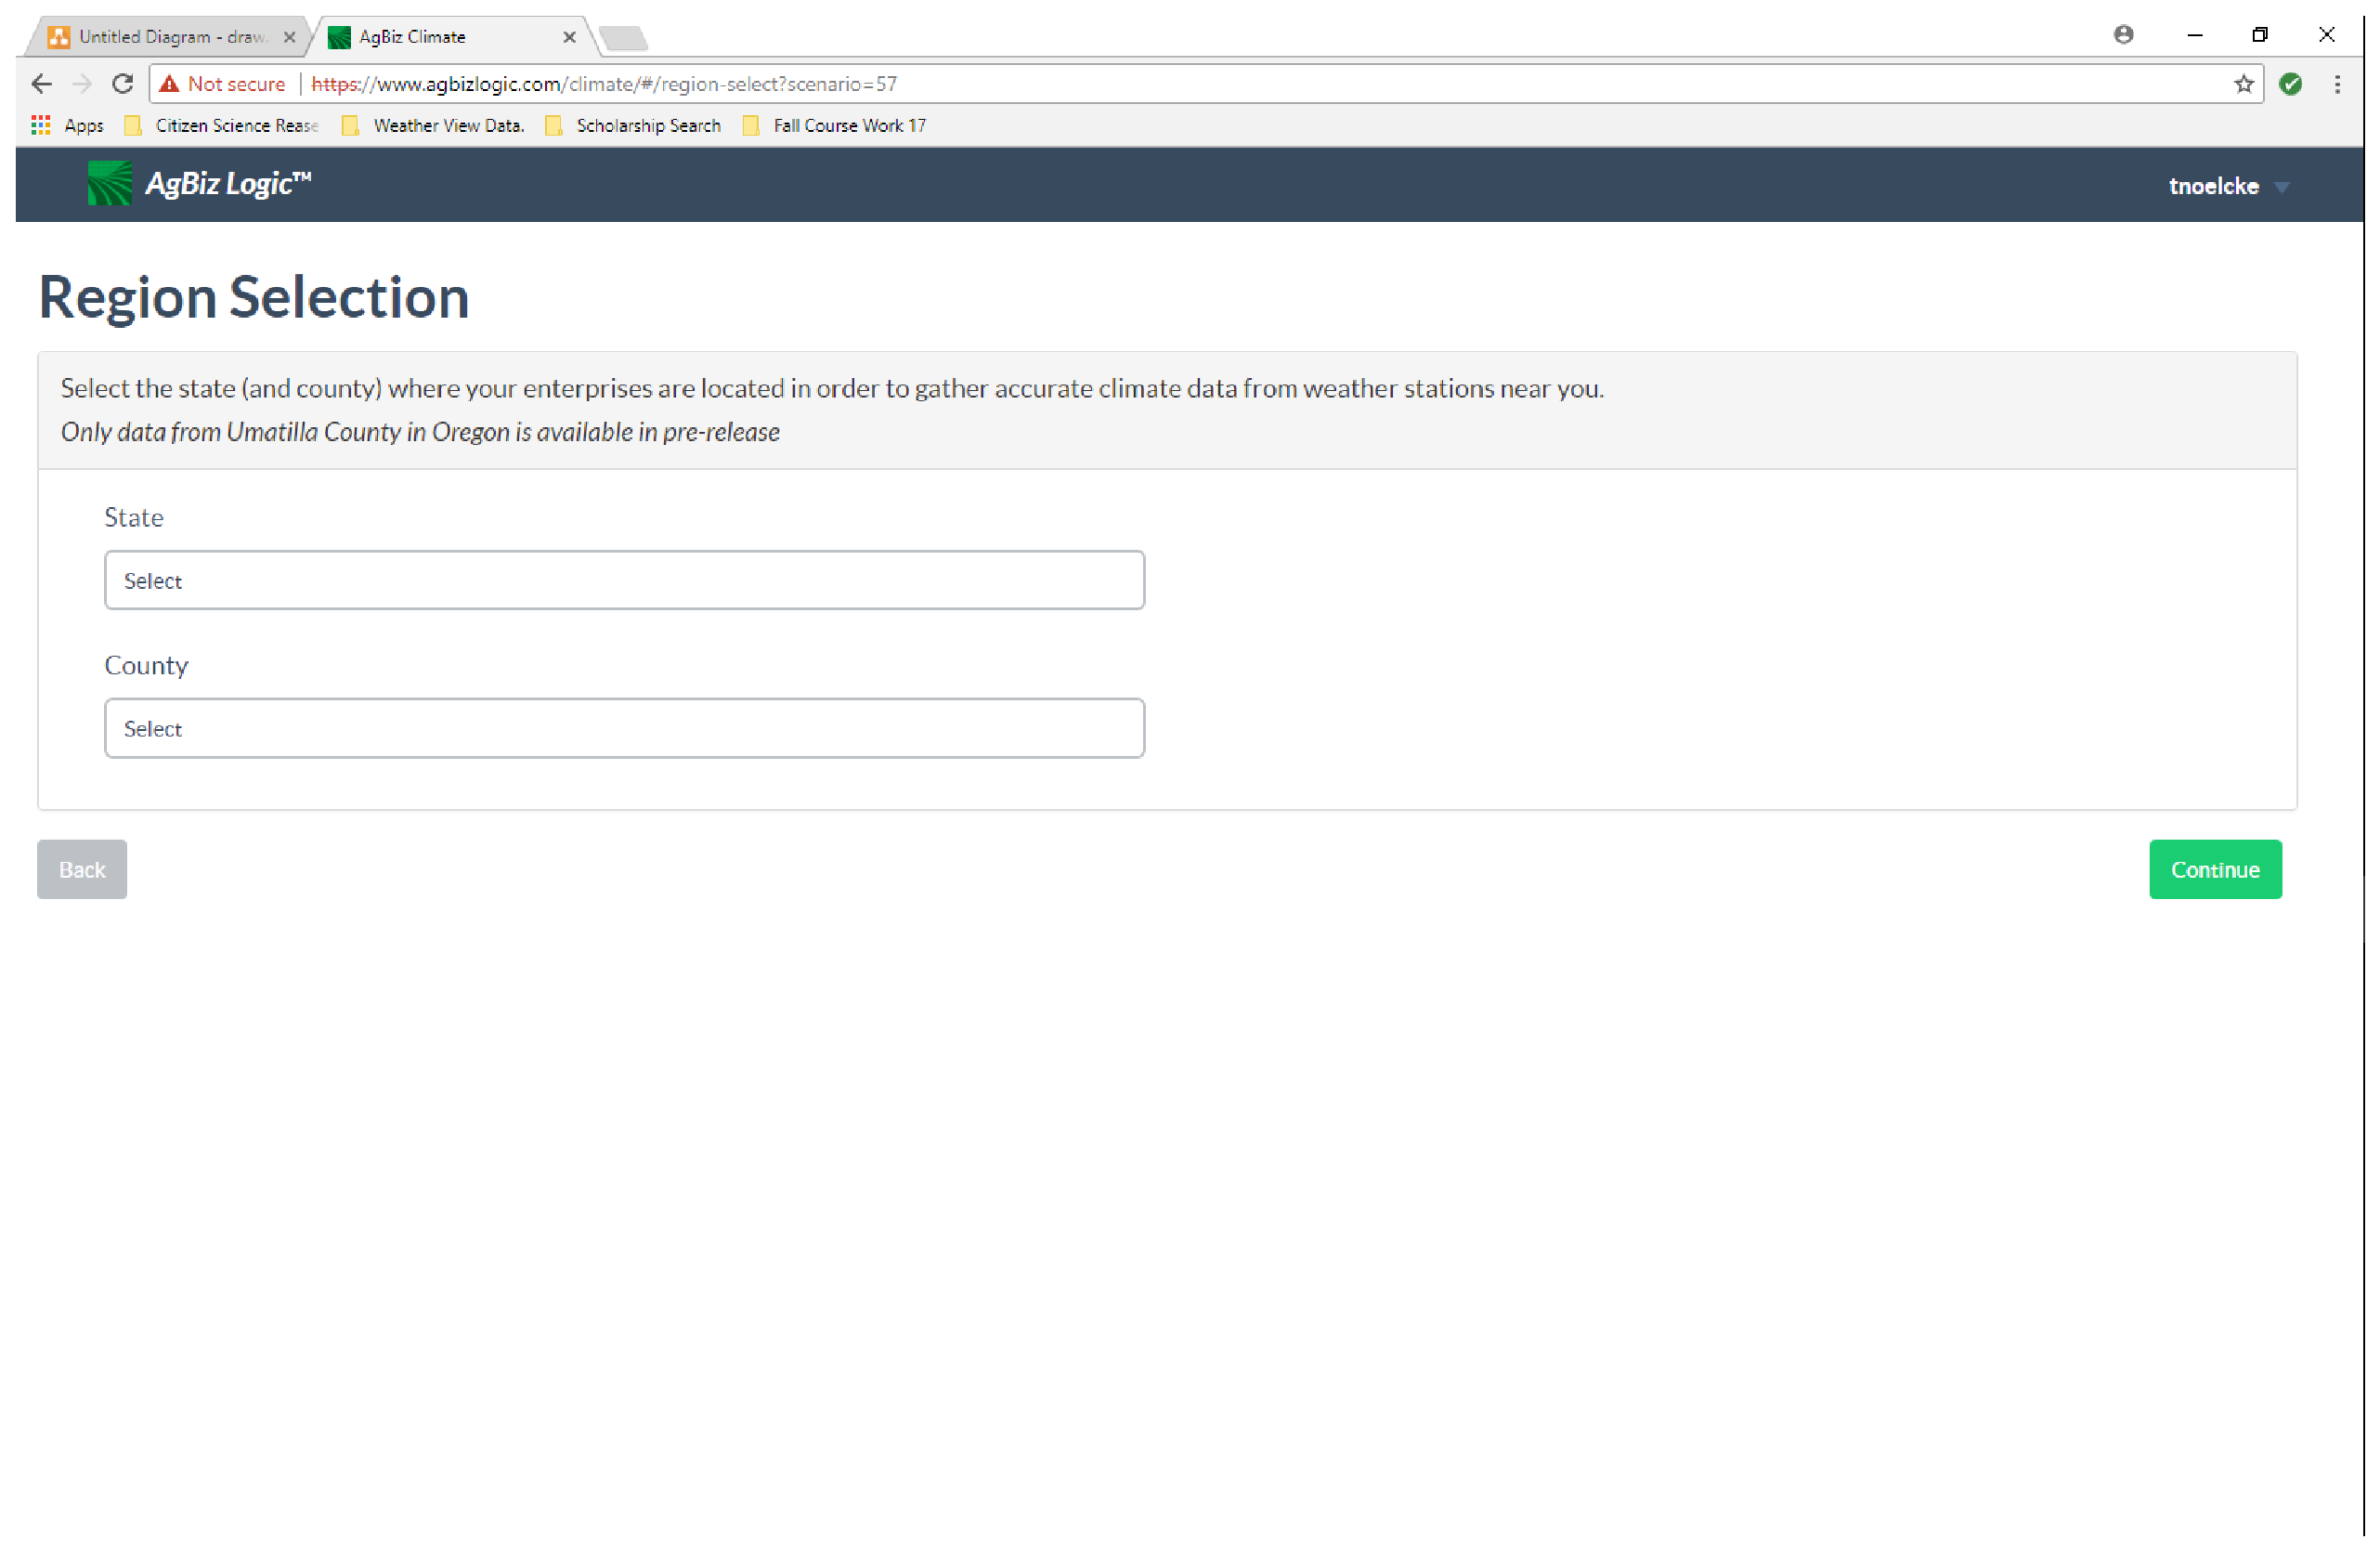
\includegraphics[width=\linewidth]{Figures/SelectStateAndCounty.eps}
						\caption{Allows User to select location}
						\label{figure3.3}
					\end{figure}

					After clicking continue the user will be taken to the plots for the location they selected. This page will initially have the 7 month average precipitation plot selected as the default. However, the user can select from four options via a drop down menu. Changing what is selected in the drop down menu will change which plot is displayed. Once the user has reviewed the plots they can then enter in how much they think their yield will be effected based on the climate data. A prototype of this page is shown below in figure 3.4.\\
					
					\begin{figure}
						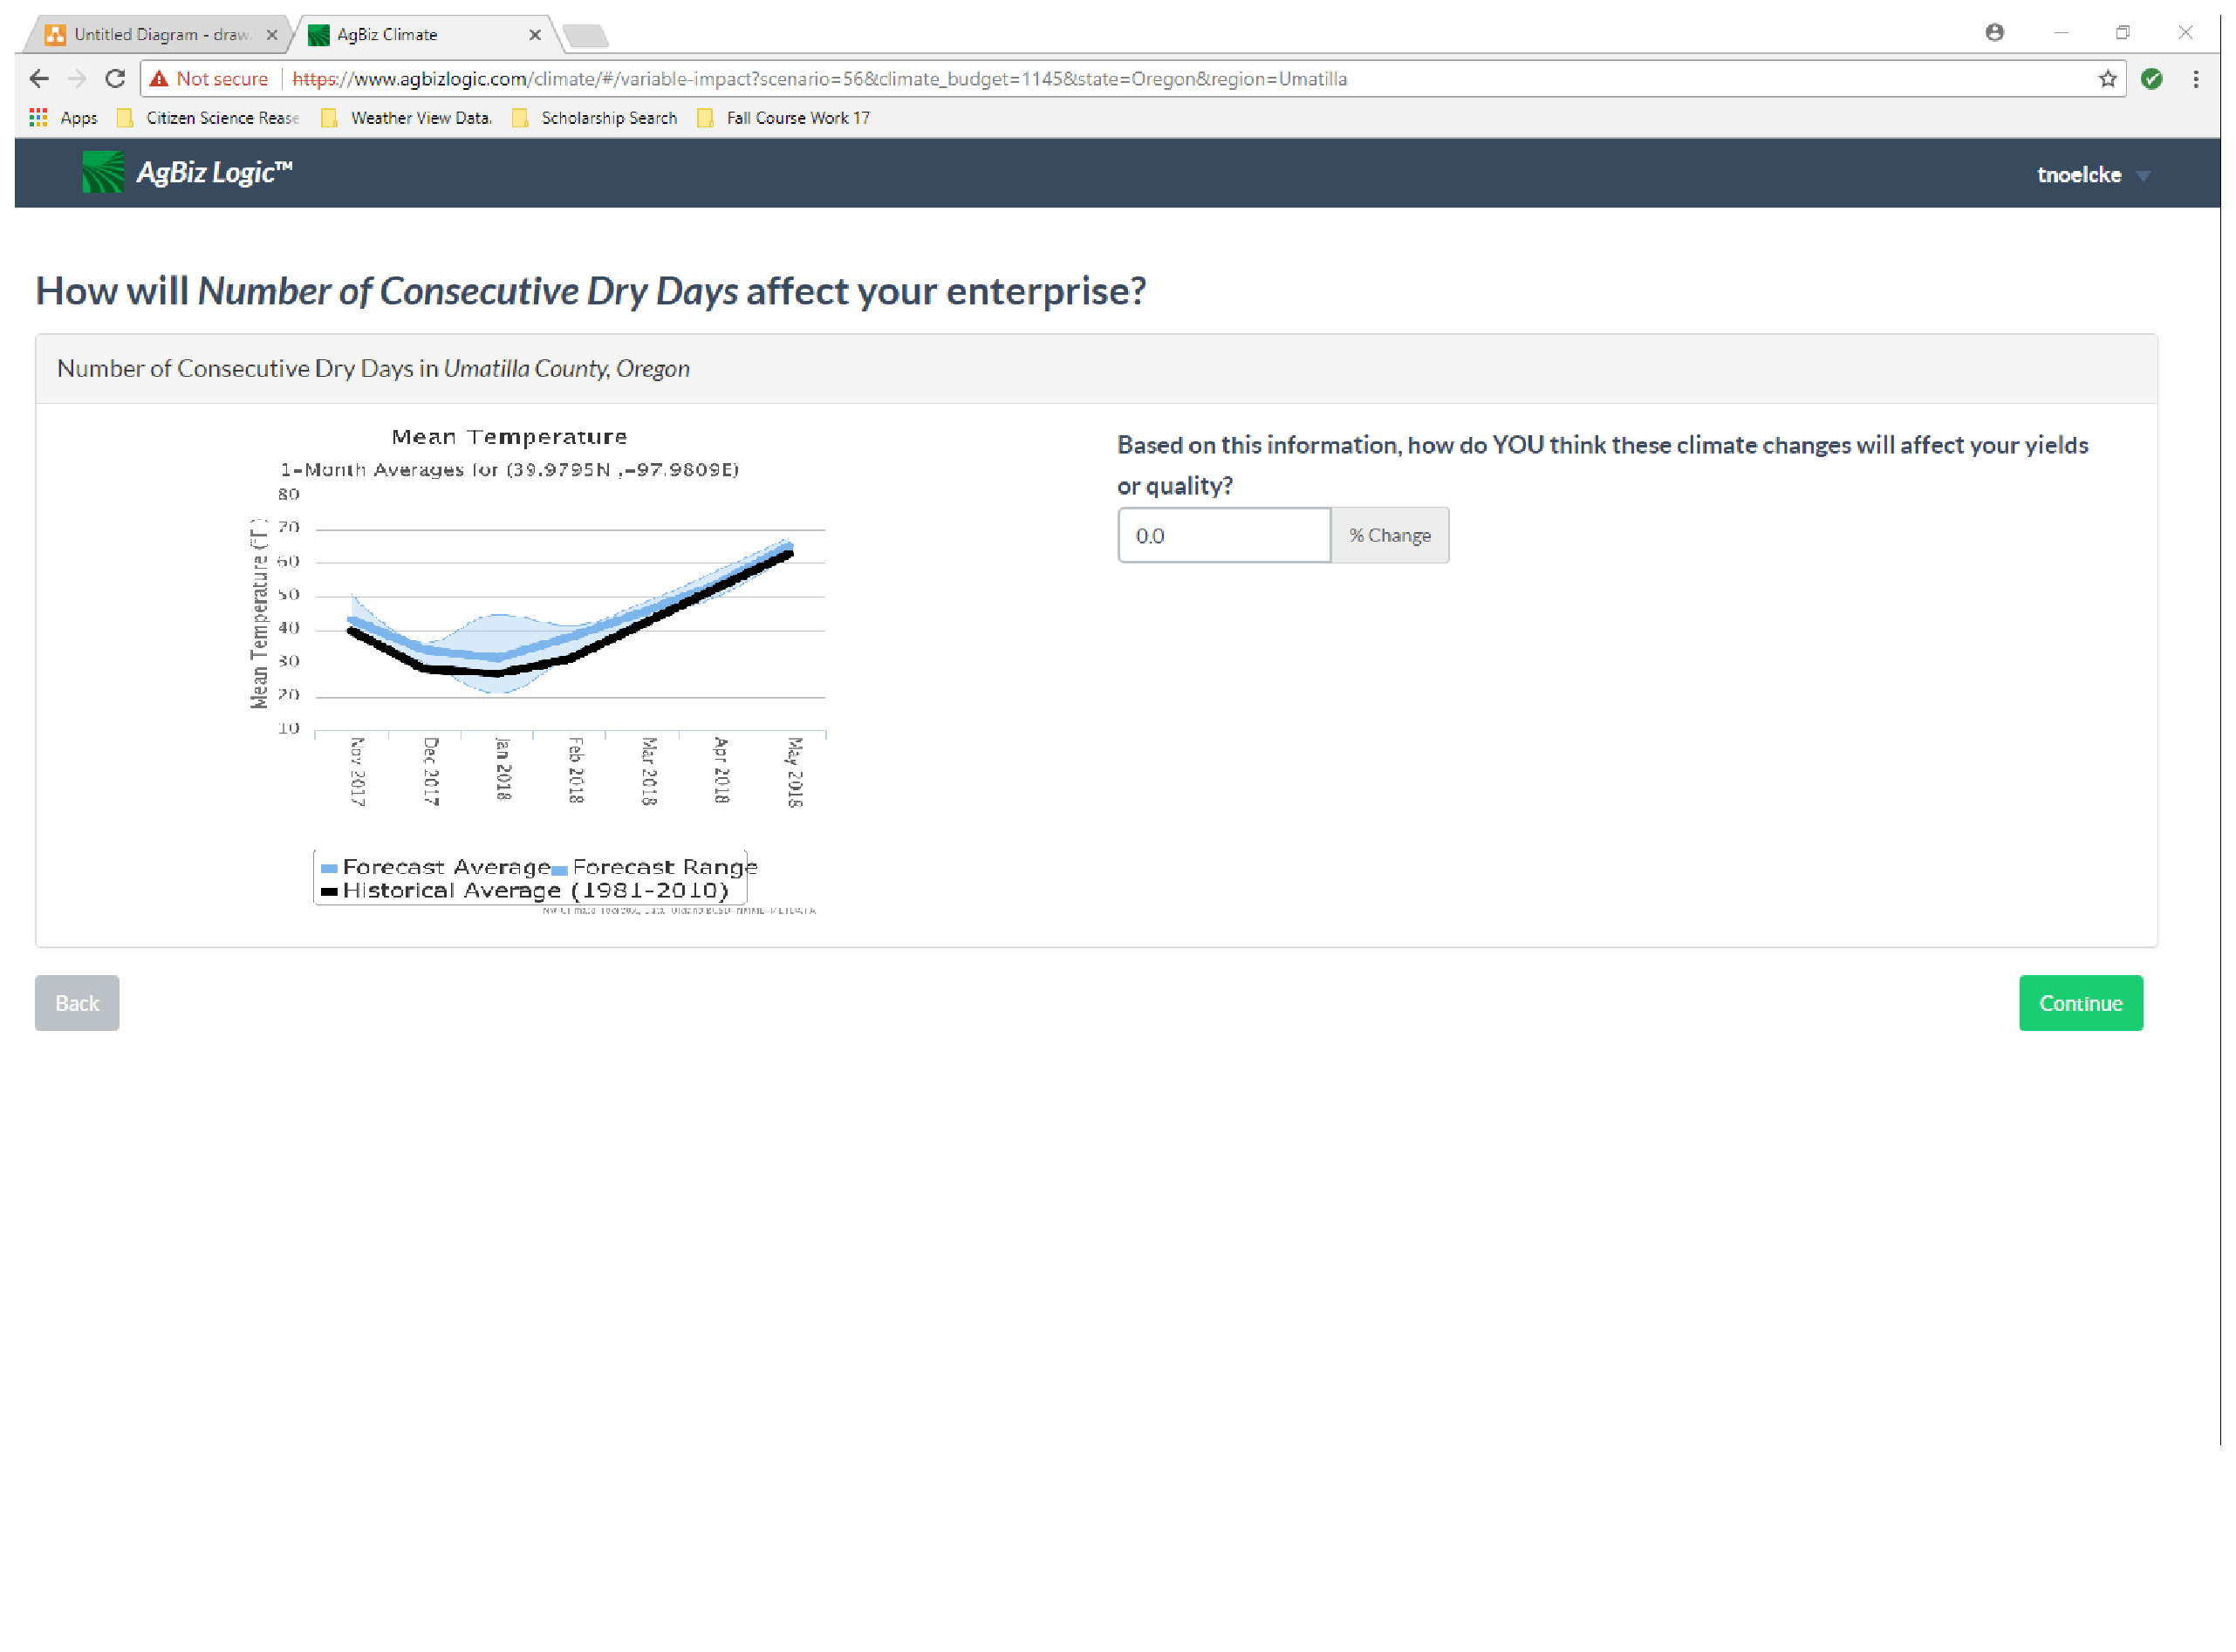
\includegraphics[width=\linewidth]{Figures/ChartPage.eps}
						\caption{Displays the Data in a plot}
						\label{figure3.4}
					\end{figure}

					Next the user will be directed to the budget review page. This page will display a summary of the budget. The summary of the budget will include Income, General Cash Costs and A total summary of the budget. This page will allow the user to adjust the cost per unit, input costs, and quantity sold and will adjust their budget in near real time. This page will also allow the user to remove or add inputs to their general costs. This page will also allow the user to save their budget and output it as a PDF. A prototype of this page is shown below in figure 3.5 (Not yet available)\\
					
					\begin{figure}
						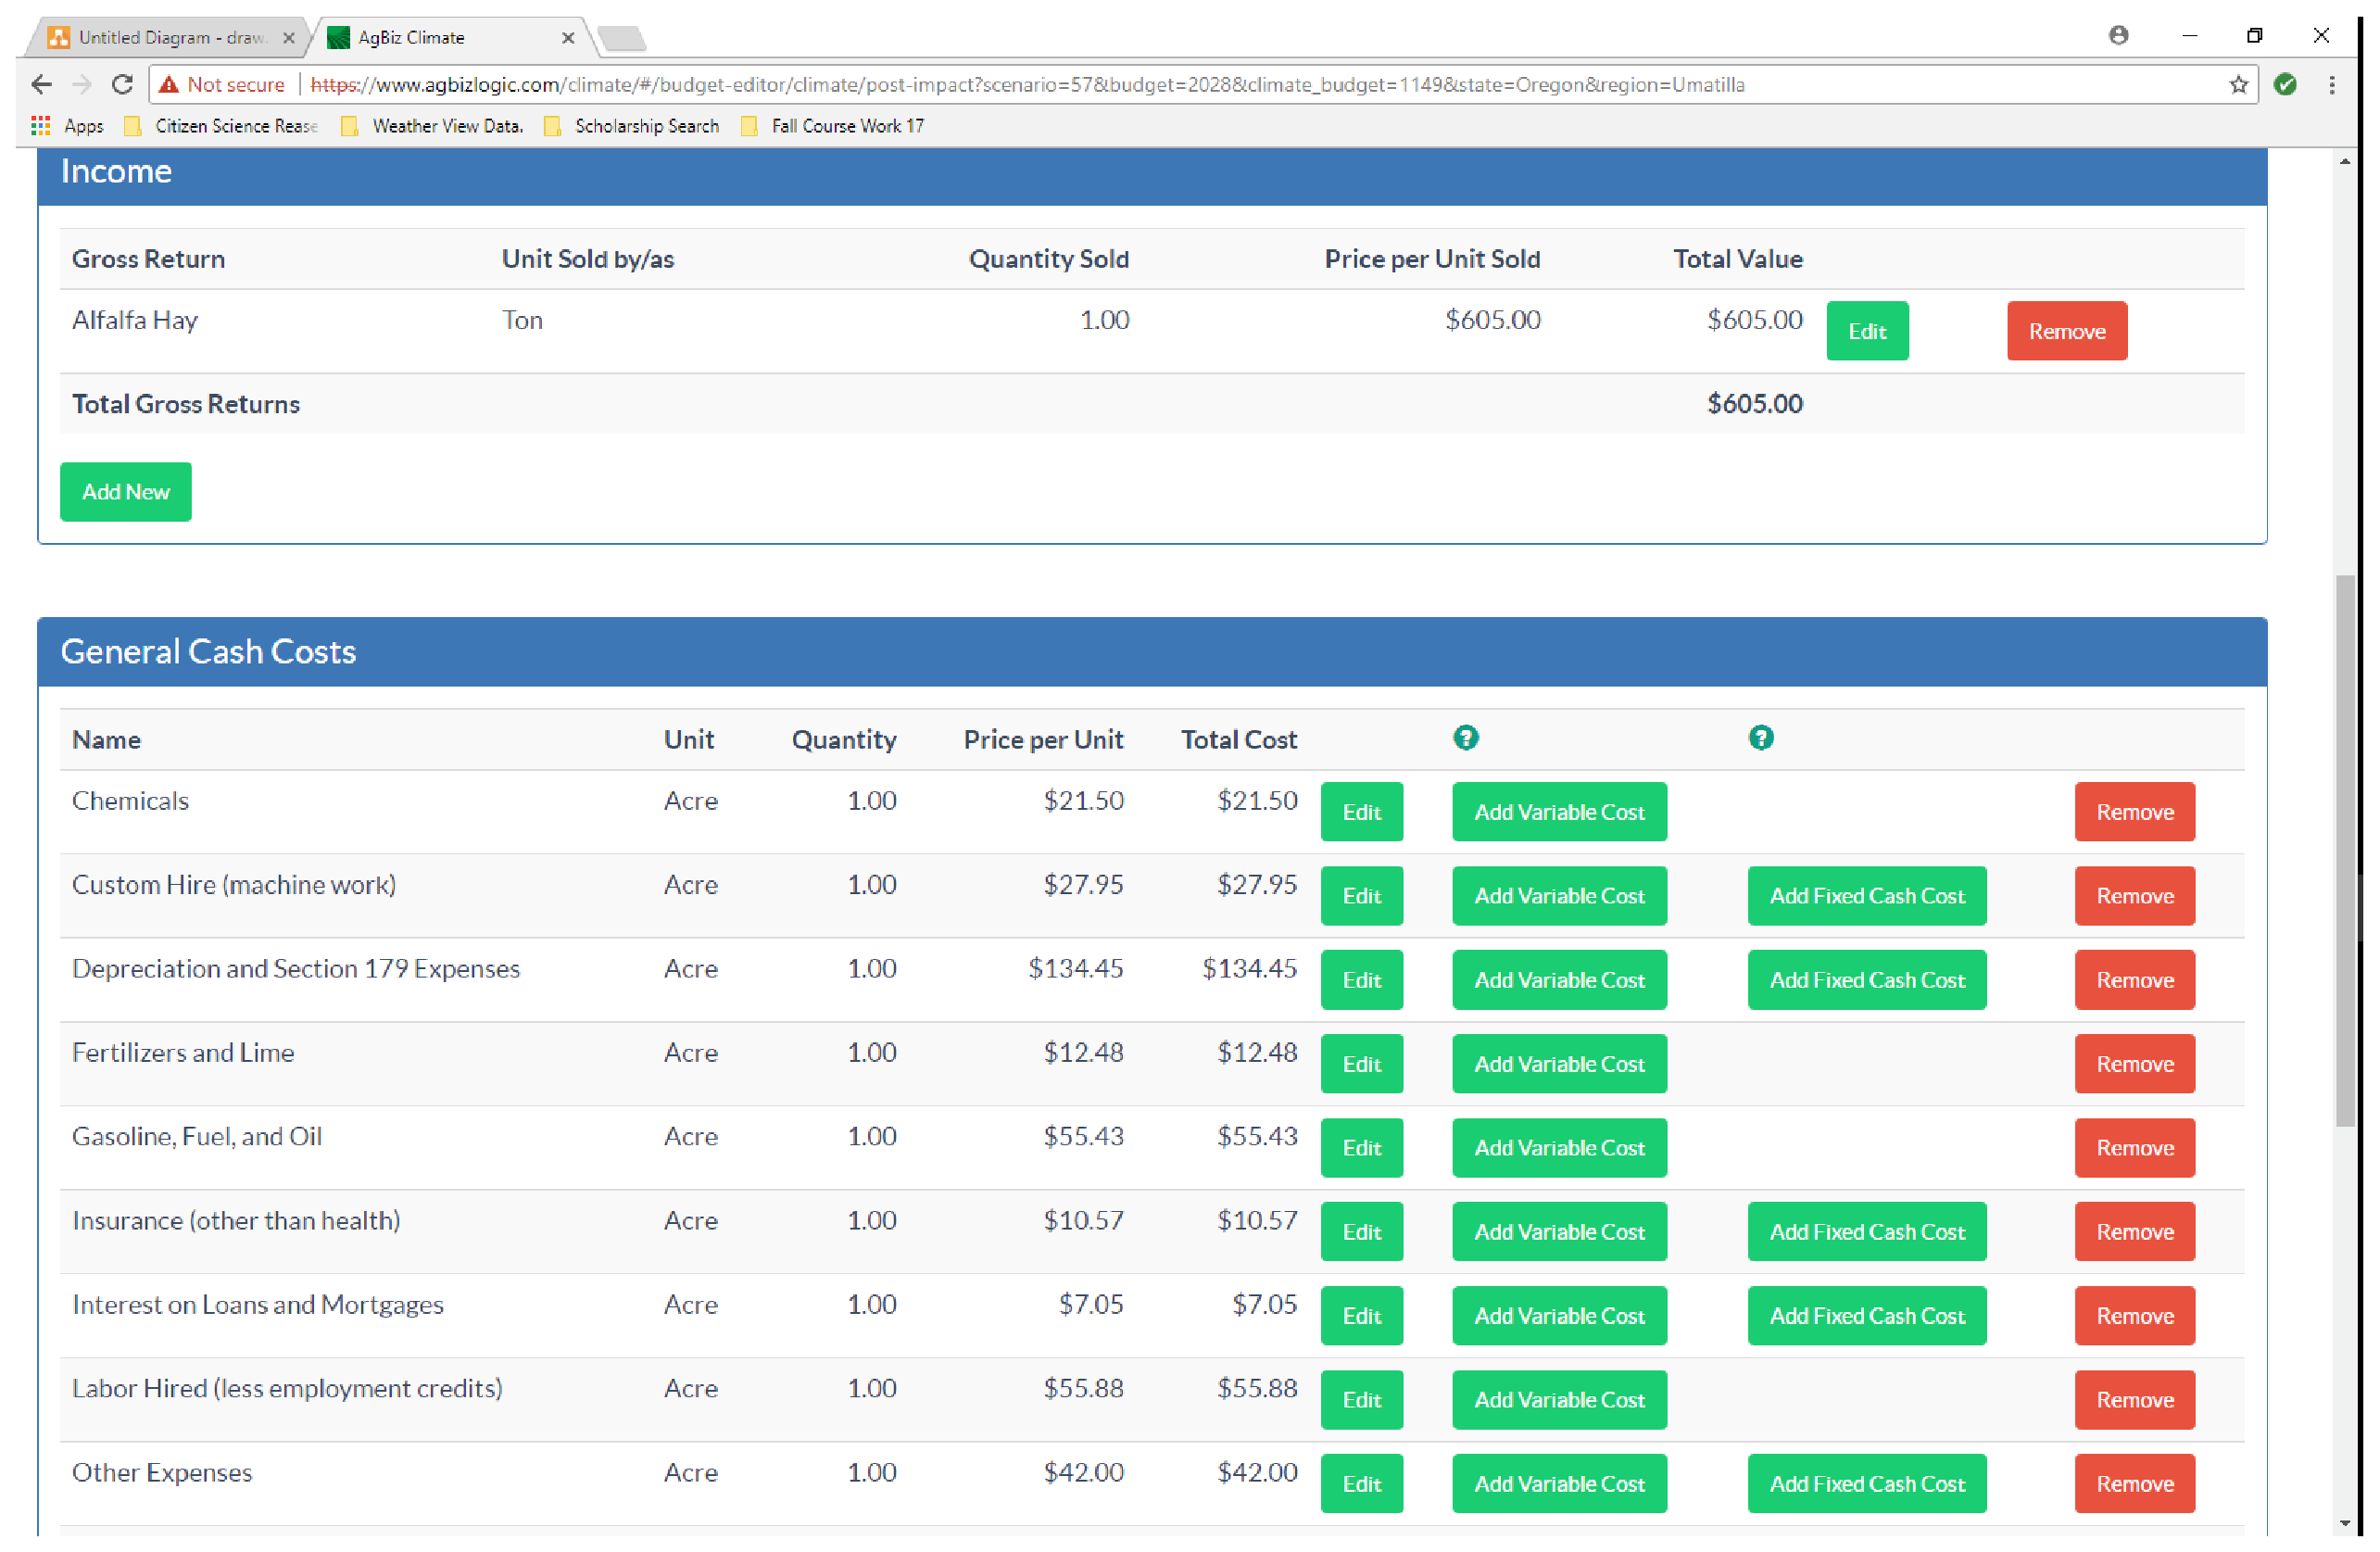
\includegraphics[width=\linewidth]{Figures/BudgetReivew.eps}
						\caption{Allows user to view their budget}
						\label{figure3.5}
					\end{figure}

        \subsubsection{Hardware Interfaces}
					This project requires no designed hardware and the hardware this system is running on is managed by the Operating system as a result no hardware interfaces are necessary. Additionally the connection the the NWCTB is managed over the network and requires no hardware interface.\\

        \subsubsection{Software Interface}
					There are several software interfaces in this application, one between the back end and the front end, one between the back end and the Database and finally a software interface between our RESTFUl API and the NWCTB. The majority of the connections between the front end and the back end are managed for us the the current \textit{AgBiz Logic} system. However, we will still need to connect our API to the back end to provide the data from the NWCTB. To make this connection we will use a RESTFULL API. This will allow for the back end code to make a direct call to our API to extract the data.\\
					We will also need a connection between the NWCTB and our API. At the time of writing this document we have not received any information from the NWCTB regarding the API they have promised access too. However, We do know that we will need to authenticate the connection with the data base, send a request and then receive the result. Authenticating the connection will involve some sort of hand shake where we pass the NWCTB a key. Once we authenticate the connection we can then send a request. A request will contain a variety of information including a location for which we want the data. Once we have sent the request we will then wait for the response and accept the data. We may also need to store this data is a data base. If this is necessary we will need an additional software interface between the database and the API.\\

        \subsubsection{Communications Interfaces}
					This project will require communication between its various parts. One key lane of communication is between the front end and back end of the application. Another key lane of communication will be between the NWCTB and our API. Most of the communication between components will be carried out through HTTP requests. These are managed by the operating system and will not effect the way our application works.\\


		\subsection{Functional Requirements}
			In this Section we will list and discuss the functional requirements for this project. Each functional requirement shall have an ID, Title, Description and Dependencies. The ID shall be unique for each requirement. The description will give a detailed expiation of the requirement. The dependencies section will list the requirements that will need to be complete before starting work on that requirement.\\


			%Decided to go with functional requirements instead of user stories because
			%it will make our Gantt Chart much easier to draft.
			\subsubsection{Functional Requirements For API}
					\paragraph{Functional Requirement 1.1}
						\textbf{ID: FR1.1} \hfill \break
						Title: Request for Users Location Data\hfill \break
						Description: The API shall take an HTTP Post request with the users State and County as parameters. Upon receiving the HTTP Post request the API will strip the parameters off the Request and store the values in variables for later use.\\
						Dependencies: FR2.1\hfill \break

					\paragraph{Functional Requirement 1.2}
						\textbf{ID: FR1.2}\hfill \break
						Title: Transforming Users Location data.\hfill \break
						Description: The API shall take the users Sate and county information and transform it into latitude and longitude. It shall then store the results in a variable for later use.\\
						Dependencies: FR1.1 and FR2.1\hfill \break

					\paragraph{Functional Requirement 1.3}
						\textbf{ID: FR1.3}\hfill \break
						Title: NWCTB Authentication
						Description: The API shall authenticate the connection with the NWCTB by sending a request to connect to the NWCTB. This request will include a validation key to ensure that the connection is valid.\\
						Dependencies: None.\hfill \break

					\paragraph{Functional Requirement 1.4}
						\textbf{ID: FR1.4}\hfill \break
						Title: Requesting data\hfill \break
						Description: After the correct user information has been gathered and the connection with the NWCTB has been authenticated the API shall send a request to the NWCTB API for the information the user requested. This request shall be made via an HTTP Get request.\\
						Dependencies: FR1.1, FR1.2, FR1.3 and FR2.1\hfill \break

					\paragraph{Functional Requirement 1.5}
						\textbf{ID: FR1.5}\hfill \break
						Title: Receive Response from NWCTB\hfill \break
						Description: After sending the request for the data to the NWCTB API the API shall wait for a response to the request. Once a response has been send the API will receive this response through an HTTP Response. If the request for the user data results in an error the API shall send the appropriate response code along with a useful error message. This shall be done through an HTTP Post response.\\
						Dependencies: FR1.1, FR1.2, FR1.3, FR1.4 and FR1.5.\hfill \break

					\paragraph{Functional Requirement 1.6}
							\textbf{ID: FR1.6}\hfill \break
							Title: Processing the Data to JSON\hfill \break
							Description: Once the request has been successfully received the API shall process the raw data in the response body of the HTTP response sent by the NWCTB API. The raw data shall be placed into a JSON object and useful labels shall be applied to the JSON object so it can be easily displayed later.\\
							Dependencies: FR1.1, FR1.2, FR1.3, FR1.4, FR1.5 and FR2.1\hfill \break

					\paragraph{Functional Requirement 1.7}
						\textbf{ID: FR1.7}\hfill \break
						Title: Send the Data to the Front End\hfill \break
						Description: Once the data has been place into a JSON object and formatted the API shall send the resulting data to the front end application so it can be displayed. This shall be done via an HTTP Post response. The JSON object that contains the formatted data shall be placed in the response body. The appropriate headers for the Response shall be set to indicate that the response contains a JSON object.\\
						Dependencies: FR1.1, FR1.2, FR1.3, FR1.4, FR1.5, FR1.6 and FR2.1\hfill \break

			\subsubsection{Functional Requirements For Front End}

				\paragraph{Functional Requirement 2.1}
					\textbf{ID: FR2.1}\hfill \break
					Title: Landing Page.\hfill \break
					Description: Upon loading the \textit{AgBizClimate} application the user will be directed to a loading page this page will allow the user to select between the short term climate tool and the long term climate tool.\\
					Dependencies: None.\hfill \break

				\paragraph{Functional Requirement 2.2}
					\textbf{ID: FR2.2}\hfill \break
					Title: Request data from API\hfill \break
					Description: After selecting the short term data tool the user will be directed to a page where they will be required to enter the location they would like to analyze. This page will require the user to first enter a state via a drop down menu and then a county via a drop down menu. Clicking the continue button will send an HTTP request to the API for the climate data for the location the user requested. The Front end will then wait for a response to the request sent to the API. This request shall be made through an HTTP Post request.\\
					Dependencies: FR2.1\hfill \break

				\paragraph{Functional Requirement 2.3}
					\textbf{ID: FR2.3}\hfill \break
					Title: Plot the Data\hfill \break
					Description: After the API processes the request for the data for the location the the user specified the front end will receive the response from the API. The front end shall then take the data out of the response body and use a plotting library to plot the data and display it to the user.\\
					Dependencies: FR1.1, FR1.2, FR1.3, FR1.4, FR1.5, FR, 1.6, FR1.7, FR2.1 and FR2.2\hfill \break

				\paragraph{Functional Requirement 2.4}
					\textbf{ID: FR2.4}\hfill \break
					Title: Entering Adjustments to yield\hfill \break
					Description: Once the data has been plotted and displayed the the user front end shall allow the user to make adjustments to the expected yield of the crop they are analyzing. This shall be done via a text box. The user input shall be limited to a decimal number with no more than one decimal place.\\
					Dependencies: FR1.1, FR1.2, FR1.3, FR1.4, FR1.5, FR, 1.6, FR1.7, FR2.1, FR2.2 and FR2.3\hfill \break

				\paragraph{Functional Requirement 2.5}
					\textbf{ID: FR2.5}\hfill \break
					Title: Redirect To Budget Tool.\hfill \break
					Description: Once the user has entered the adjustments to the yield for the crop they are analyzing they shall then be redirected to the existing \textit{AgBizClimate} budgeting tool. This tool will be sent the data they entered in the previous step and shall reflect the adjustments to yield that they made.\\
					Dependencies: FR1.1, FR1.2, FR1.3, FR1.4, FR1.5, FR, 1.6, FR1.7, FR2.1, FR2.2, FR2.3 and FR2.4\hfill \break
			\subsubsection{Functional Requirements for Testing}
				\paragraph{Functional Requirement 3.1}
				\textbf{ID: FR3.1}\hfill \break
				Title: Unit Tests For API Routes.
				Description: We shall write unit tests to cover 100 percent of our API routes. Each route shall have a test case that is non-trivial and seeks to emulate how the route will be used by the application. These test cases shall test that the correct response is returned from each API route.\\
				Dependencies: FR1.1, FR1.2, FR1.3, FR1.4, FR1.5, FR1.6 and FR2.1\hfill \break
				\paragraph{Functional Requirement 3.2}
				\textbf{ID: FR3.2}\hfill \break
				Title: Unit Tests for User Actions on Front End \hfill \break
				Description: We shall provide unit tests for the various user actions on the front end of the application. The front end tests shall ensure that clickable objects on the page perform the correct action. We shall provide tests for all clickable objects that redirect the application to another page. Our tests shall ensure that if a clickable action is clicked that the correct action is taken for each clickable object.\\
				Dependencies:  FR1.1, FR1.2, FR1.3, FR1.4, FR1.5, FR, 1.6, FR1.7, FR2.1, FR2.2, FR2.3, FR2.4 and FR2.5\hfill \break
				\paragraph{Functional Requirement 3.3}
				\textbf{ID: FR3.3}\hfill \break
				Title: Unit Tests for Budget Save \hfill \break
				Description: We shall provide unit tests that ensure that the budget is being correctly saved once the user is all done making adjustments to their budget. This test case shall ensure that the values sent to the back-end of the application are posted to the database. The test will also ensure that the values posted in the database are correct.\\
				Dependencies:  FR1.1, FR1.2, FR1.3, FR1.4, FR1.5, FR, 1.6, FR1.7, FR2.1, FR2.2, FR2.3, FR2.4 and FR2.5\hfill \break

    \subsection{Performance Requirements}
    	In this section we will list the performance metrics for our application. This performance metrics will describe acceptable performance for our application. Each requirement will have a title and a description that provides details for how that metric will be measured.
				\subsubsection{Performance Metric 1}
               	\textbf{Title:} Run Time Performance \hfill \break
                Our application shall provide the plotted data in a reasonable amount of time 100 percent of the time. Reasonable being defined as less than 5 seconds. This time shall be measured from the time the user presses the next button after selecting their state and county to the time the web page is loaded with the plot being displayed.\\
                \subsubsection{Performance Metric 2}
                \textbf{Title:} Reliability \hfill \break
                Our application shall provide the correct result to the user 100 percent of the time. This result can include an error if the user enters a location that doesn't exist or if the data the user request is unavailable.\\

    \subsection{Design Constraints}
			The constraints of this project can be divided into two parts. Software constraints and hardware constraints. In this section we will discuss these constraints.\\
			\subsubsection{Software Constraints}
				This project shall be implemented using Django, Angular JS and SQL databases. What we add must also be done using Django, Angular JS and SQL.\\

				Additionally, what we create must work with the the existing \textit{AgBiz Logic} system. This means we will be forced to use software interfaces and databases that have already been implemented that we have no control over.\\

			\subsubsection{Hardware Constraints}
				Another factor that will effect how our software works is the hardware that this system is running on. The hardware this system runs on has already been determined and is managed by the university. We don't expect that the hardware will affect our project. However, we have no control over the hardware the \textit{AgBiz Logic} system is running on.\\

    \subsection{Other Requirements}
				This section will cover any additional information pertinent to this project but not covered in other sections.\\
				\subsubsection{Stretch Requirements}
				In this section we will discuss requirements not apart of our contract with our client. These goals will not be required as apart of this project but are objectives that we would like to complete.\\
					\paragraph{Stretch Requirement 1.1}
						Title: Location Via a Map\\
						Description: In requirement 2.2 instead of using two drop down menus to select the location the user would be able to use a pin on a map of the US to select their location. This would be done through an existing library that would allow us to take a pin on a map and produce a latitude and longitude.\\
						Dependencies: FR2.1 and FR2.2\\
\section{Gantt Chart}

Here we will place our Gantt Chart. Will get completed before Friday.\\




\end{document}

